% ============================================================
% 8-point radix-2 DIT FFT diagram
%
% Usage:
%   \fft{0}
%   \fft{8}
%   \fft{16}
%
% The argument is the first input/output index.
% ============================================================

\newcommand{\fft}[3]{%
% \begin{tikzpicture}[scale=0.5]

% Store the first index
\pgfmathtruncatemacro{\base}{#1}
\pgfmathtruncatemacro{\xpos}{#2}
\pgfmathtruncatemacro{\ypos}{#3}

% ------------------------------------------------------------
% Input labels (bit-reversed order)
% ------------------------------------------------------------

\foreach \i/\v in {
    0/0,
    1/4,
    2/2,
    3/6,
    4/1,
    5/5,
    6/3,
    7/7
}{
    \pgfmathtruncatemacro{\idx}{\base+\v}
    \node (fft-\base-x-\i) at (0+\xpos,-\i+\ypos)
        {$x[\idx]$};
}

% ------------------------------------------------------------
% Stage nodes
% ------------------------------------------------------------

\foreach \i in {0,...,7}{
    \node[
        circle,
        fill=gray!70,
        inner sep=0,
        minimum size=.1cm
    ] (fft-\base-s0-\i) at (1+\xpos,-\i+\ypos) {};

    \node[
        circle,
        fill=gray!70,
        inner sep=0,
        minimum size=.1cm
    ] (fft-\base-s1-\i) at (2+\xpos,-\i+\ypos) {};

    \node[
        circle,
        fill=gray!70,
        inner sep=0,
        minimum size=.1cm
    ] (fft-\base-s2-\i) at (3+\xpos,-\i+\ypos) {};

    \node[
        circle,
        fill=gray!70,
        inner sep=0,
        minimum size=.1cm
    ] (fft-\base-s3-\i) at (4+\xpos,-\i+\ypos) {};
}

% ------------------------------------------------------------
% Input -> Stage 0
% ------------------------------------------------------------

% \foreach \i in {0,...,7}{
%     \draw[draw=gray!70]
%         (fft-\base-x-\i)
%         -- (fft-\base-s0-\i);
% }

% ------------------------------------------------------------
% Stage 1: butterflies of size 2
% ------------------------------------------------------------

\draw[draw=gray!70] (fft-\base-s0-0) -- (fft-\base-s1-0);
\draw[draw=gray!70] (fft-\base-s0-0) -- (fft-\base-s1-1);
\draw[draw=gray!70] (fft-\base-s0-1) -- (fft-\base-s1-0);
\draw[draw=gray!70] (fft-\base-s0-1) -- (fft-\base-s1-1);

\draw[draw=gray!70] (fft-\base-s0-2) -- (fft-\base-s1-2);
\draw[draw=gray!70] (fft-\base-s0-2) -- (fft-\base-s1-3);
\draw[draw=gray!70] (fft-\base-s0-3) -- (fft-\base-s1-2);
\draw[draw=gray!70] (fft-\base-s0-3) -- (fft-\base-s1-3);

\draw[draw=gray!70] (fft-\base-s0-4) -- (fft-\base-s1-4);
\draw[draw=gray!70] (fft-\base-s0-4) -- (fft-\base-s1-5);
\draw[draw=gray!70] (fft-\base-s0-5) -- (fft-\base-s1-4);
\draw[draw=gray!70] (fft-\base-s0-5) -- (fft-\base-s1-5);

\draw[draw=gray!70] (fft-\base-s0-6) -- (fft-\base-s1-6);
\draw[draw=gray!70] (fft-\base-s0-6) -- (fft-\base-s1-7);
\draw[draw=gray!70] (fft-\base-s0-7) -- (fft-\base-s1-6);
\draw[draw=gray!70] (fft-\base-s0-7) -- (fft-\base-s1-7);

% ------------------------------------------------------------
% Stage 2: butterflies of size 4
% ------------------------------------------------------------

\draw[draw=gray!70] (fft-\base-s1-0) -- (fft-\base-s2-0);
\draw[draw=gray!70] (fft-\base-s1-0) -- (fft-\base-s2-2);
\draw[draw=gray!70] (fft-\base-s1-2) -- (fft-\base-s2-0);
\draw[draw=gray!70] (fft-\base-s1-2) -- (fft-\base-s2-2);

\draw[draw=gray!70] (fft-\base-s1-1) -- (fft-\base-s2-1);
\draw[draw=gray!70] (fft-\base-s1-1) -- (fft-\base-s2-3);
\draw[draw=gray!70] (fft-\base-s1-3) -- (fft-\base-s2-1);
\draw[draw=gray!70] (fft-\base-s1-3) -- (fft-\base-s2-3);

\draw[draw=gray!70] (fft-\base-s1-4) -- (fft-\base-s2-4);
\draw[draw=gray!70] (fft-\base-s1-4) -- (fft-\base-s2-6);
\draw[draw=gray!70] (fft-\base-s1-6) -- (fft-\base-s2-4);
\draw[draw=gray!70] (fft-\base-s1-6) -- (fft-\base-s2-6);

\draw[draw=gray!70] (fft-\base-s1-5) -- (fft-\base-s2-5);
\draw[draw=gray!70] (fft-\base-s1-5) -- (fft-\base-s2-7);
\draw[draw=gray!70] (fft-\base-s1-7) -- (fft-\base-s2-5);
\draw[draw=gray!70] (fft-\base-s1-7) -- (fft-\base-s2-7);

% ------------------------------------------------------------
% Stage 3: butterflies of size 8
% ------------------------------------------------------------

\draw[draw=gray!70] (fft-\base-s2-0) -- (fft-\base-s3-0);
\draw[draw=gray!70] (fft-\base-s2-0) -- (fft-\base-s3-4);
\draw[draw=gray!70] (fft-\base-s2-4) -- (fft-\base-s3-0);
\draw[draw=gray!70] (fft-\base-s2-4) -- (fft-\base-s3-4);

\draw[draw=gray!70] (fft-\base-s2-1) -- (fft-\base-s3-1);
\draw[draw=gray!70] (fft-\base-s2-1) -- (fft-\base-s3-5);
\draw[draw=gray!70] (fft-\base-s2-5) -- (fft-\base-s3-1);
\draw[draw=gray!70] (fft-\base-s2-5) -- (fft-\base-s3-5);

\draw[draw=gray!70] (fft-\base-s2-2) -- (fft-\base-s3-2);
\draw[draw=gray!70] (fft-\base-s2-2) -- (fft-\base-s3-6);
\draw[draw=gray!70] (fft-\base-s2-6) -- (fft-\base-s3-2);
\draw[draw=gray!70] (fft-\base-s2-6) -- (fft-\base-s3-6);

\draw[draw=gray!70] (fft-\base-s2-3) -- (fft-\base-s3-3);
\draw[draw=gray!70] (fft-\base-s2-3) -- (fft-\base-s3-7);
\draw[draw=gray!70] (fft-\base-s2-7) -- (fft-\base-s3-3);
\draw[draw=gray!70] (fft-\base-s2-7) -- (fft-\base-s3-7);

% ------------------------------------------------------------
% Output labels
% ------------------------------------------------------------

\foreach \i in {0,...,7}{
    \pgfmathtruncatemacro{\idx}{\base+\i}
    \node (fft-\base-X-\i) at (5+\xpos,-\i+\ypos)
        {$X[\idx]$};
}

% ------------------------------------------------------------
% Stage 3 -> Output
% ------------------------------------------------------------

% \foreach \i in {0,...,7}{
%     \draw[draw=gray!70]
%         (fft-\base-s3-\i)
%         -- (fft-\base-X-\i);
% }

% \end{tikzpicture}
}

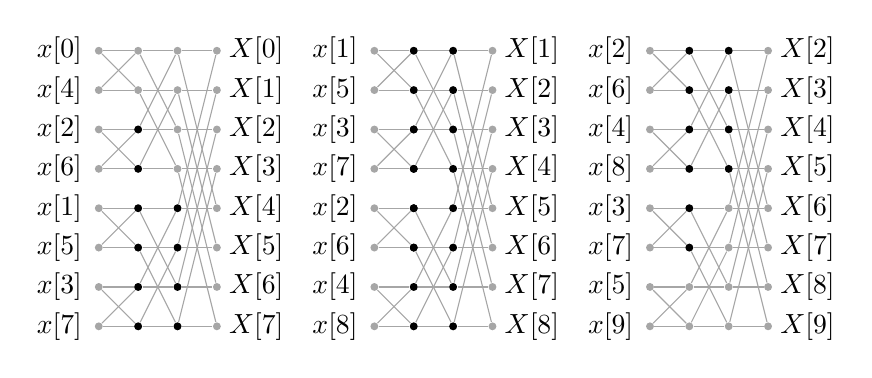
\begin{tikzpicture}[scale=0.5]
    \fft{0}{0}{0}
    \fft{1}{7}{0}
    \fft{2}{14}{0}

    % ------------------------------------------------------------
    % base0 vs base1
    % ------------------------------------------------------------

    \node<2-5>[circle, fill=black, inner sep=0, minimum size=.1cm] at (fft-0-s1-2) {};
    \node<2-5>[circle, fill=black, inner sep=0, minimum size=.1cm] at (fft-0-s1-3) {};
    \node<2-5>[circle, fill=black, inner sep=0, minimum size=.1cm] at (fft-1-s1-4) {};
    \node<2-5>[circle, fill=black, inner sep=0, minimum size=.1cm] at (fft-1-s1-5) {};

    \node<3-5>[circle, fill=black, inner sep=0, minimum size=.1cm] at (fft-0-s1-4) {};
    \node<3-5>[circle, fill=black, inner sep=0, minimum size=.1cm] at (fft-0-s1-5) {};
    \node<3-5>[circle, fill=black, inner sep=0, minimum size=.1cm] at (fft-1-s1-0) {};
    \node<3-5>[circle, fill=black, inner sep=0, minimum size=.1cm] at (fft-1-s1-1) {};
    
    \node<4-5>[circle, fill=black, inner sep=0, minimum size=.1cm] at (fft-0-s1-6) {};
    \node<4-5>[circle, fill=black, inner sep=0, minimum size=.1cm] at (fft-0-s1-7) {};
    \node<4-5>[circle, fill=black, inner sep=0, minimum size=.1cm] at (fft-1-s1-2) {};
    \node<4-5>[circle, fill=black, inner sep=0, minimum size=.1cm] at (fft-1-s1-3) {};
    
    \node<5-5>[circle, fill=black, inner sep=0, minimum size=.1cm] at (fft-0-s2-4) {};
    \node<5-5>[circle, fill=black, inner sep=0, minimum size=.1cm] at (fft-0-s2-5) {};
    \node<5-5>[circle, fill=black, inner sep=0, minimum size=.1cm] at (fft-0-s2-6) {};
    \node<5-5>[circle, fill=black, inner sep=0, minimum size=.1cm] at (fft-0-s2-7) {};
    
    \node<5-5>[circle, fill=black, inner sep=0, minimum size=.1cm] at (fft-1-s2-0) {};
    \node<5-5>[circle, fill=black, inner sep=0, minimum size=.1cm] at (fft-1-s2-1) {};
    \node<5-5>[circle, fill=black, inner sep=0, minimum size=.1cm] at (fft-1-s2-2) {};
    \node<5-5>[circle, fill=black, inner sep=0, minimum size=.1cm] at (fft-1-s2-3) {};
    
    % ------------------------------------------------------------
    % base1 vs base2
    % ------------------------------------------------------------

    \node<6-9>[circle, fill=black, inner sep=0, minimum size=.1cm] at (fft-1-s1-2) {};
    \node<6-9>[circle, fill=black, inner sep=0, minimum size=.1cm] at (fft-1-s1-3) {};
    \node<6-9>[circle, fill=black, inner sep=0, minimum size=.1cm] at (fft-2-s1-4) {};
    \node<6-9>[circle, fill=black, inner sep=0, minimum size=.1cm] at (fft-2-s1-5) {};

    \node<7-9>[circle, fill=black, inner sep=0, minimum size=.1cm] at (fft-1-s1-4) {};
    \node<7-9>[circle, fill=black, inner sep=0, minimum size=.1cm] at (fft-1-s1-5) {};
    \node<7-9>[circle, fill=black, inner sep=0, minimum size=.1cm] at (fft-2-s1-0) {};
    \node<7-9>[circle, fill=black, inner sep=0, minimum size=.1cm] at (fft-2-s1-1) {};
    
    \node<8-9>[circle, fill=black, inner sep=0, minimum size=.1cm] at (fft-1-s1-6) {};
    \node<8-9>[circle, fill=black, inner sep=0, minimum size=.1cm] at (fft-1-s1-7) {};
    \node<8-9>[circle, fill=black, inner sep=0, minimum size=.1cm] at (fft-2-s1-2) {};
    \node<8-9>[circle, fill=black, inner sep=0, minimum size=.1cm] at (fft-2-s1-3) {};
    
    \node<9-9>[circle, fill=black, inner sep=0, minimum size=.1cm] at (fft-1-s2-4) {};
    \node<9-9>[circle, fill=black, inner sep=0, minimum size=.1cm] at (fft-1-s2-5) {};
    \node<9-9>[circle, fill=black, inner sep=0, minimum size=.1cm] at (fft-1-s2-6) {};
    \node<9-9>[circle, fill=black, inner sep=0, minimum size=.1cm] at (fft-1-s2-7) {};
    
    \node<9-9>[circle, fill=black, inner sep=0, minimum size=.1cm] at (fft-2-s2-0) {};
    \node<9-9>[circle, fill=black, inner sep=0, minimum size=.1cm] at (fft-2-s2-1) {};
    \node<9-9>[circle, fill=black, inner sep=0, minimum size=.1cm] at (fft-2-s2-2) {};
    \node<9-9>[circle, fill=black, inner sep=0, minimum size=.1cm] at (fft-2-s2-3) {};
\end{tikzpicture}